%%%%%%%%%%%%%%%%%%%%%%%%%%%%%%%%%%%%%%%%%%%%%%%%%%%%%%%%
%%%%%%%%%%%%%%%%%%%%%%%%%%%%%%%%%%%%%%%%%%%%%%%%%%%%%%%%
%%%%%%%%%%%%%%%%%%%%%%%%%%%%%%%%%%%%%%%%%%%%%%%%%%%%%%%%
\section{Legendrian links and their Lagrangian fillings}\label{sec:Legendrian_links_Lagrangian_fillings}

The object of this section is to explain how to transition from the algebraic and diagrammatic aspects of Demazure weaves, as presented in Part I, to the geometric context of contact and symplectic topology. We focus on two constructions:\\

\begin{enumerate}
    \item Given a positive braid word $\beta$, we obtain a Legendrian link $\La_\beta\sse(S^3,\xi_\std)$ in the standard contact 3-sphere, cf.~\Cref{ssec:Legendrian_link_beta}, and explain how the braid variety $X(\beta)$ can be understood in terms of such a Legendrian link, cf.~\Cref{ssec:braid_varieties_Legendrian_links}.\\
    \item After reviewing Lagrangian fillings in \Cref{ssec:Lagrangian_fillings}, we then construct in \Cref{ssec:Lagrangian_filling_from_AG} embedded exact Lagrangian surfaces $L\sse(\D^4,\la_\std)$ by studying certain algebraic curves in $\C^2$ with purely imaginary periods. Such a class of Lagrangian surfaces, and the way in which they can be plotted, provide a compelling motivation to introduce weave diagrams $\wb$ and later construct Lagrangian surfaces $L_\w$ from them.
\end{enumerate}

\begin{comment}

\noindent A central geometric goal in low-dimensional contact and symplectic topology is to \textcolor{blue}{classify embedded exact Lagrangian surfaces with a fixed Legendrian boundary link, up to compactly supported Hamiltonian isotopy}. Part of the motivation to study Demazure weaves and cluster structures on braid varieties is that new results in symplectic topology can be obtained towards that classification.\\

\noindent In fact, from a hopeful viewpoint, I conjecture that the classification of such Lagrangian surfaces bounding $\La_\beta$ is given by the cluster seeds of the cluster algebra structure on the coordinate ring of functions of the braid variety $X(\beta)$. We will present and discuss results providing some evidence towards that conjecture. For now, we start building the geometric objects from the ground up and relate them to the diagrammatic calculus of Demazure weaves from \Cref{sec:diagrammatic_weaves}.
\end{comment}


%%%%%%%%%%%%%%%%%%%%%%%%%%%%%%%%%%%%%%%%%%%%%%%%%%%%%%%%
%%%%%%%%%%%%%%%%%%%%%%%%%%%%%%%%%%%%%%%%%%%%%%%%%%%%%%%%
%%%%%%%%%%%%%%%%%%%%%%%%%%%%%%%%%%%%%%%%%%%%%%%%%%%%%%%%
\subsection{The Legendrian link of a positive braid word}\label{ssec:Legendrian_link_beta}

Let $\beta$ be a positive braid word. The first step towards geometry is to consider a Legendrian link $\La_\beta\sse(S^3,\xi_\std)$ associated to $\beta$. A Legendrian link embedded in the 3-sphere $S^3$ is a particular type of smooth link. Specifically, it is a link constrained to a tangency condition with respect to the 2-plane distribution $\xi_\std$ given by the complex tangencies of the unit sphere
$$S^3=\{(z_1,z_2)\in\C^2: |z_1|^2+|z_2|^2=1\}\sse\C^2,\qquad \xi_\std:=TS^3\cap i(TS^3).$$

\begin{definition}[Legendrian links]\label{def:legendrian_link} Let $\La\sse S^3$ be a smooth link embedded in the 3-sphere. By definition, $\La$ is said to be a Legendrian link if $T\La\sse\xi_\std$, i.e.~if the tangent line $T_p\La\sse T_pS^3$ at every point $p\in\La$ belongs to the 2-plane of complex tangencies $T_pS^3\cap i(T_pS^3)$.\\

\noindent By definition, two Legendrian links $\La_0,\La_1\sse (S^3,\xi_\std)$ are said to be Legendrian isotopic if there exists a 1-parametric family $\La_t\sse(S^3,\xi_\std)$ of Legendrian links with $t\in[0,1]$.\sbs
\end{definition}

\begin{center}
	\begin{figure}[h!]
		\centering
		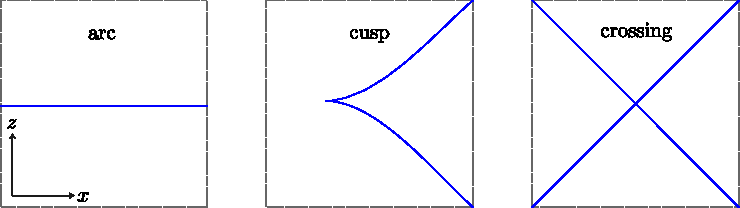
\includegraphics[scale=0.85]{figures/Front_Arc_Cusp_Crossing_R3.pdf}
		\caption{The generic 3 planar pieces of a front $\ff\sse\R^2_{x,z}$ of a Legendrian link $\La\sse(\R^3,\xi_\std)$.}
		\label{fig:Front_Arc_Cusp_Crossing_R3}
	\end{figure}
\end{center}

In the same manner that smooth links in the 3-sphere can be studied by using link diagrams in the plane, Legendrian links can be studied by using front diagrams. In contrast to link diagrams, fronts do not need to specify the overcrossing and undercrossing information. For our purposes, a front for a Legendrian link can be defined as an immersed curve $\mathfrak{f}$ in the plane $\R^2_{x,z}$, except for finitely many simple cusp singularities, having no vertical tangencies. See \Cref{fig:Front_Arc_Cusp_Crossing_R3_Example1} for two instances of fronts. Thus a front is locally built of the three types of pieces depicted in \Cref{fig:Front_Arc_Cusp_Crossing_R3}, consisting of arcs, simple cusps and crossings, none of which ever acquires a vertical tangent line. These are locally modeled as
$$\mbox{arc}:=\{z=0\},\quad \mbox{cusp}:=\{x^3=z^2\},\quad\mbox{crossing}:=\{(x-z)(x+z)=0\}.$$

\noindent From a front $\mathfrak{f}\sse \R^2_{x,z}$ we can construct a Legendrian link:

\begin{definition}[Legendrian link from a front]\label{def:legendrian_link_from_front} Let $\mathfrak{f}\sse \R^2_{x,z}$ be a front, then the Legendrian link $\La_\mathfrak{f}$ is
\begin{equation}\label{def:leglink_from_front}
\La_\mathfrak{f}:=\{(x,y,z)\sse\R^3: y=\dd_x z(x)\}
\end{equation}
where at each point we have locally expressed $\mathfrak{f}$ as the graph of a function $z(x)$.\sbs
\end{definition}

\noindent A few comments on \Cref{def:legendrian_link_from_front}:

\begin{enumerate}
    \item The condition $y=\dd_x z(x)$ guarantees that $\La_\mathfrak{f}$ is tangent to the 2-plane distribution $\xi:=\ker\{dz-ydx\}\sse T\R^3$ in $\R^3$. This is relevant to \Cref{def:legendrian_link} because the complement of a point in $(S^3,\xi_\std)$ is isomorphic\footnote{The precise term is contactomorphic, see \cite[Chapter 2]{Geiges08}.} to $(\R^3,\ker\{dz-ydx\})$. In particular, by considering the one-point compactification $\R^3\sse S^3$, we can always think of $\La_\mathfrak{f}$ as a Legendrian link in $(S^3,\xi_\std)$, which we will still denote by $\La_\ff$. In a sense, \Cref{def:legendrian_link_from_front} is the analogue in contact topology to the fact in smooth topology that a link diagram in the plane determines a unique link in $\R^3$, up to smooth isotopy.\\

    \item For \eqref{def:leglink_from_front}, it is possible to always locally express the restriction of the $z$-coordinate in $\R^2_{x,z}$ to $\mathfrak{f}$ as a function $z|_{\ff}=z(x)$ because of the implicit function theorem, as there are no vertical tangencies in $\mathfrak{f}$. In addition, the Legendrian link $\La_\ff\sse\R^3$ is a smooth link. Indeed, at a cusp singularity $\{x^3=z^2\}$ of $\ff$, as in \Cref{fig:Front_Arc_Cusp_Crossing_R3} (center), the lift can be smoothly parametrized by $\gamma(t)=(t^2,3t/2,t^3)$. Similarly, at a crossing $\{(x-z)(x+z)=0\}$ of $\ff$ the crossing point lifts to two distinct points $(0,\pm 1,0)$ in $\R^3$. These points are distinguished in $\R^3$ by the $y$-coordinates, which measure the slopes of the branches at the crossing point in $\ff\sse\R^2_{x,z}$.\\
\end{enumerate}

\begin{center}
	\begin{figure}[h!]
		\centering
		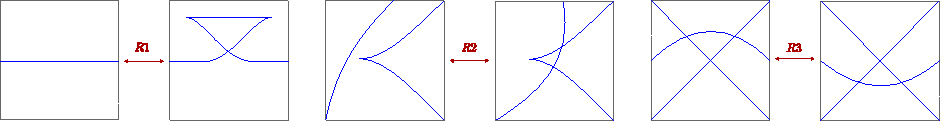
\includegraphics[width=\textwidth]{figures/Front_Arc_Cusp_Crossing_R3_3Reidemeister.pdf}
		\caption{Legendrian Reidemeister moves in the front projection. Each of these moves can be realized by a Legendrian isotopy. Conversely, in $(\R^3,\xi_\std)$ every Legendrian isotopy is itself isotopic to a Legendrian isotopy whose front projections are exactly a sequence of these three Reidemeister moves. There are symmetric versions of these moves which we always implicitly include: R1 upside-down, R2 with the cusp pointing east.}
		\label{fig:Front_Arc_Cusp_Crossing_R3_Reidemeister}
	\end{figure}
\end{center}

In smooth topology, the Reidemeister theorem states that two link diagrams give rise to two smoothly isotopic links in $\R^3$ if and only if the link diagrams differ by certain moves, known as the Reidemeister moves. Similarly, a Legendrian enhancement of the Reidemeister theorem states that given two fronts $\ff_0,\ff_1$, then $\La_{\ff_0}\simeq \La_{\ff_1}$ are Legendrian isotopic if and only if $\ff_0$ and $\ff_1$ can be connected through the three Legendrian Reidemeister moves, as depicted in \Cref{fig:Front_Arc_Cusp_Crossing_R3_Reidemeister}, and a compactly supported ambient smooth isotopy where the fronts do not acquire vertical tangencies.

\noindent Remarkably, there are typically many Legendrian links that are not Legendrian isotopic even if their underlying smooth links are smoothly isotopic. For instance, \Cref{fig:Front_Arc_Cusp_Crossing_R3_Example1} depicts two Legendrian fronts $\ff_0,\ff_1$ such that $\La_{\ff_0}$ and $\La_{\ff_1}$ are smoothly isotopic but not Legendrian isotopic.

\begin{center}
	\begin{figure}[h!]
		\centering
		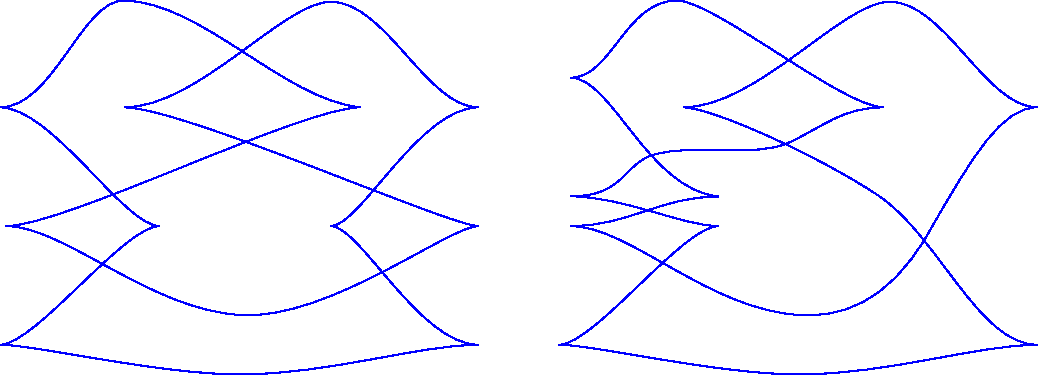
\includegraphics[scale=0.5]{figures/Front_Arc_Cusp_Crossing_R3_Examples1.pdf}
		\caption{Two fronts for two Legendrian knots $\La\sse(\R^3,\xi_\std)$, fronts drawn in $\R^2_{x,z}$. The smooth type of both these knots in $\R^3$ is that of $m(5_2)$, the mirror of the three twist knot: the only 5-crossing knot apart from the $(2,5)$-torus knot. These Legendrian knots are smoothly isotopic but not Legendrian isotopic, as first proven in \cite[Example 4.4]{Chekanov}.}
		\label{fig:Front_Arc_Cusp_Crossing_R3_Example1}
	\end{figure}
\end{center}

For our purposes, it will suffice to focus on the following class of Legendrian links:

\begin{fdef}
[Legendrian link associated to $\beta$]\label{def:Legendrian_from_braid} Let $\beta\in \brn$ be a positive braid word and $\delta(\beta)$ its Demazure product. By definition, $\La_\b\sse(\R^3,\xi_\std)$ is the Legendrian link defined by the front in \cref{fig:FrontsBeta} (left). It is said to be the $(-1)$-closure of $\beta\delta(\beta)$.\sbs
\end{fdef}
\vspace{0.2cm}

See \Cref{fig:FrontsBeta} (right) for an instance of \Cref{def:Legendrian_from_braid}. A key connection between braid varieties and symplectic topology is that the braid variety $X(\beta)$, as discussed in \Cref{sec:weaves_braid_varieties}, is intimately related to the Legendrian link $\La_\beta$, as we will momentarily explain.

\begin{center}
	\begin{figure}[h!]
		\centering
		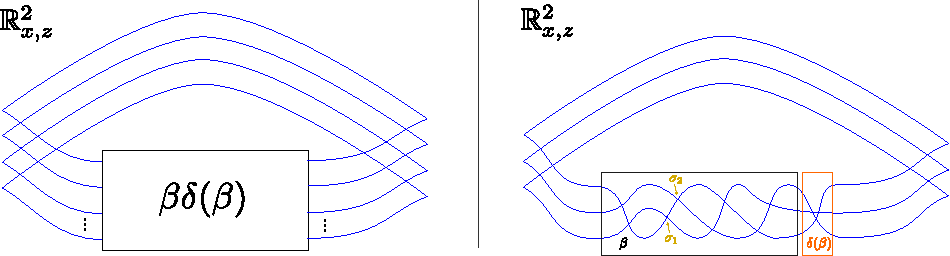
\includegraphics[scale=0.9]{figures/FrontsBetaCDM.pdf}
		\caption{(Left) The front in $\R^2_{x,z}$ for $\La_\beta\sse(\R^3,\ker\{dz-ydx\})$ referred to as the $(-1)$-closure of $\beta\delta(\beta)$. (Right) The front of the Legendrian link $\La_\beta$ for the 3-stranded positive braid word $\beta=\s_2\s_1(\s_1\s_2)^3$.}
		\label{fig:FrontsBeta}
	\end{figure}
\end{center}

\noindent A few comments on \Cref{def:Legendrian_from_braid} are in order:

\begin{enumerate}
    \item If two braid words $\beta_1,\beta_2$ differ by braid moves $\s_i\s_{i+1}\s_i\to\s_{i+1}\s_i\s_{i+1}$, then $\La_{\beta_1}\simeq\La_{\beta_2}$ are Legendrian isotopic by the third Legendrian Reidemeister move, as in \Cref{fig:Front_Arc_Cusp_Crossing_R3_Reidemeister} (right). Similarly, if they differ by a commutation $\s_i\s_j\to\s_j\s_i$, $|i-j|\geq2$, then $\La_{\beta_1}\simeq\La_{\beta_2}$ are Legendrian isotopic, as there is an ambient planar isotopy that relates these fronts. Therefore, the Legendrian isotopy type of $\La_\beta$ only depends on the underlying braid element $[\beta]$, i.e.~it is independent of the choice of braid word $\beta$ for $[\beta]$.\\

    \item The literature has also featured the rainbow closure of a positive braid word $\beta$, as depicted in \cref{fig:FrontsBeta2} (right), cf.~\cite[Section 6.5]{STZ2017}. It is an exercise to show that this is an instance of a $(-1)$-closure, specifically the $(-1)$-closure of $w_0\beta w_0$, cf.~\cref{fig:FrontsBeta2}. Also, the smooth type of $\La_\beta$ is that of the smooth link typically associated in smooth topology to the braid $w_0^{-1}\beta\delta(\beta) w_0^{-1}$, by closing the braid smoothly without any framing, i.e.~the 0-closure, with no twists. Briefly put, the crossings in each of the two sides of the $\beta\delta(\beta)$-box in \cref{fig:FrontsBeta} (left) are each smoothly contributing $w_0^{-1}$.\\

    \item From the viewpoint of smooth knot theory, the class of Legendrians $\La_\beta\sse(\R^3,\xi_\std)$ is reasonably broad, as it includes smooth knots in each of the three classes: torus knots, satellite knots and hyperbolic knots. Thurston's results imply that any smooth knot must be in one of these three classes, cf.~\cite[Cor.~2.5]{Thurston82}. In fact, for each of these smooth classes, there exist infinitely many Legendrian knots of the form $\La_\beta$ in such class, each not smoothly isotopic to one another, cf.~\cite[Section 6.2]{CasalsGao22}.
\end{enumerate}

\begin{center}
	\begin{figure}[h!]
		\centering
		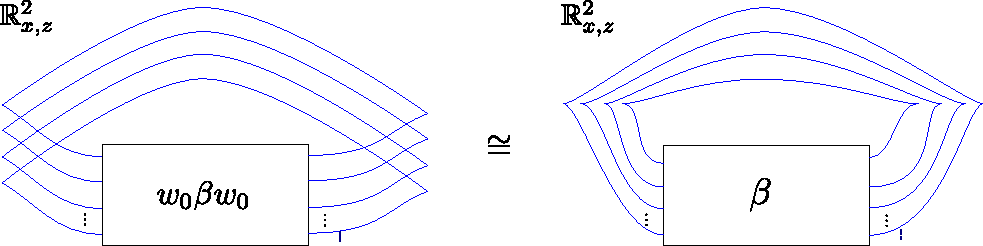
\includegraphics[scale=0.9]{figures/FrontsBeta2.pdf}
		\caption{(Left) The $(-1)$-closure of $w_0\beta w_0$, where $w_0$ is any positive braid word representing the half-twist. (Right) The rainbow closure of $\beta$, which is Legendrian isotopic to the $(-1)$-closure of $w_0\beta w_0$.}
		\label{fig:FrontsBeta2}
	\end{figure}
\end{center}

\begin{example} (1) Consider $c:=\sigma_1\ldots\sigma_{n-1}\in\Br_n^+$ and let $w_0$ be any positive braid word representing the half-twist, e.g.~$w_0=\sigma_1(\sigma_2\sigma_1)\cdots(\sigma_{n-1}\cdots\sigma_2\s_1)$. Then the Legendrian link $\La_\b$ associated to $\beta=w_0c^m$ is a Legendrian representative of the $(n,m)$-torus link. If $\gcd(n,m)=1$, then $\La_\beta$ is a knot and it is the unique max-tb Legendrian representative of the $(n,m)$-torus link. In the context of cluster algebras, these Legendrian links will be closely related to the top-dimensional positroid variety in the Grassmannian $\mbox{Gr}(n,n+m)$, cf.~\Cref{ssec:braid_varieties_examples}.(2) and \Cref{ex:simple_braidvarieties}.(2). More generally, the max-tb Legendrian representative of an algebraic knot is unique and it is of the form $\La_{w_0}\beta$ for some $\beta\in\Br_n^+$, cf.~\cite{CasalsLagSkel}.\\

\noindent (2) If $\beta=\s_1^2\s_2^2\s_1^2\s_2^2\s_1\s_2\in\mbox{Br}_3^+$, then $\La_\b$ is Legendrian isotopic to the Legendrian representative of $m(5_2)$ depicted in \cref{fig:Front_Arc_Cusp_Crossing_R3_Example1} (left). The Legendrian representative of $m(5_2)$ depicted in \cref{fig:Front_Arc_Cusp_Crossing_R3_Example1} (right) is {\it not} of the form $\La_\beta$ for any $n\in\N$ and $\beta\in\mbox{Br}_n^+$, see e.g.~\cite[Section 7.2.2]{STZ2017}.\sbs
\end{example}

%%%%%%%%%%%%%%%%%%%%%%%%%%%%%%%%%%%%%%%%%%%%%%%%%%%%%%%%
%%%%%%%%%%%%%%%%%%%%%%%%%%%%%%%%%%%%%%%%%%%%%%%%%%%%%%%%
%%%%%%%%%%%%%%%%%%%%%%%%%%%%%%%%%%%%%%%%%%%%%%%%%%%%%%%%
\subsection{Braid varieties from Legendrian links}\label{ssec:braid_varieties_Legendrian_links} A driving goal in low-dimensional contact topology is the classification of Legendrian links, up to Legendrian isotopy. Part of such classification involves showing that some Legendrian links are {\it not} Legendrian isotopic to each other. This is achieved by developing Legendrian invariants. There is now a range of such Legendrian invariants, from numerical ones, such as the Thurston-Bennequin number and the rotation number, to polynomial invariants, such as the ruling polynomial, and algebraically richer ones, including certain dg-categories and $A_\infty$-categories. Let us focus on two such invariants:\\

\begin{enumerate}
    \item {\bf The Legendrian contact dg-algebra}. For a Legendrian link $\La\sse(\R^3,\xi_\std)$ and a choice of basepoints $\tt$, this is a non-commutative dg algebra $\mathbb{A}(\La,\tt)$ whose quasi-isomorphism type only depends on the Legendrian isotopy class of $\La$ and the choice of basepoints $\tt$, cf.~\cite{Chekanov,EtnyreNg22_Survey}. For context, the dg-category of perfect dg-modules over $\mathbb{A}(\La,\tt)$ is an explicit presentation of the partially wrapped Fukaya category of $(\D^4,\la_\std)$ stopped at $\La$, cf.~\cite{EkholmLekili2023}.\\
    
    For the Legendrian links of the form $\La=\La_\beta$, as in \Cref{def:Legendrian_from_braid}, this dg algebra $\mathbb{A}(\La_\beta,\tt)$ is defined over $\Z$ and it is $\Z$-graded. An explicit presentation for $\mathbb{A}(\La_\beta,\tt)$ is given in \cite[Section 5.1]{CasalsNg22}, and its homology is reasonably understood, see e.g.~\cite[Corollary 1.1]{casals2026vanishinghigherlegendrianhomology}. In this case of $\La=\La_\beta$ we always choose the basepoints $\tt$ to be one per strand of $\beta$, and located to the right of all crossings of $\beta$, cf.~\cite[Section 5]{CasalsNg22}. To ease notation, we often abbreviate $\mathbb{A}(\La_\beta,\tt)$ to $\mathbb{A}(\La_\beta)$ since the basepoints are understood to be chosen according to this convention.\\

    \item {\bf The dg category of sheaves with singular support on $\La$}. Building on the notion of singular support of a sheaf introduced in \cite{KashiwaraSchapira_Book}, the dg category $\operatorname{Sh}_\La(\R^2)$ of (categorically) compact complexes of sheaves of $\kk$-modules on $\R^2_{x,z}$ with singular support contained in the (cone of the) Legendrian link $\La$ is a Legendrian invariant of $\La$, cf.~\cite{GKS_Quantization}. It is conjectured that $\operatorname{Sh}_\La(\R^2)$ is equivalent to the dg-category of perfect dg-modules over $\mathbb{A}(\La)$.\\
\end{enumerate}

A central connection between braid varieties and Legendrian links is as follows:\\

\begin{center}
  \fbox{%
    \begin{tabular}{l}
      \itshape The braid variety $X(\beta)$ appears naturally as a Legendrian invariant of $\La_\beta$, \\
      \itshape either via its Legendrian contact dg algebra or its dg category of sheaves.
    \end{tabular}%
  }
\end{center}
\vspace{0.1cm}
\noindent Recall that the braid variety $X(\beta)$ admits a $\T$-action as described in \Cref{sssec:braid_variety_further_symmetries}, see also \Cref{lem:torusaction_coordinates}. Specifically, the tenet above can be formalized in the following result:

\begin{theorem}[Braid varieties as Legendrian invariants]\label{thm:braid_varieties_from_Legendrian}
Let $\beta\in\brn$ be a positive braid word, $\La_\beta\sse(\R^3,\xi_\std)$ its associated Legendrian link, and $X(\beta)$ its braid variety. Then:

\begin{enumerate}[label=$(\roman*)$]
    \item There exists an isomorphism of algebraic varieties over $\Z$
    \begin{equation}\label{eq:braid_variety_dga}
    X(\beta)\cong\operatorname{Spec }\operatorname{H}_0(\mathbb{A}^{ab}(\La_\beta)) 
    \end{equation}
    
    \noindent where the right hand side denotes the $0$th homology of the abelianization $\mathbb{A}^{ab}(\La_\beta)$ of the Legendrian dg algebra $\mathbb{A}(\La_\beta)$, and it is computed with one basepoint per strand of $\beta$.\\

    \item There exists an isomorphism of algebraic stacks
    \begin{equation}\label{eq:braid_variety_sheaf}
        [X(\beta)/\T]\cong \M^{\dagger}(\operatorname{Sh}_\La(\R^2))
    \end{equation}

    \noindent where $\M^{\dagger}(\operatorname{Sh}_\La(\R^2))$ denotes the component of $\GL_1$-local systems in the 1-truncation $t_1(\M(\La_\beta))$ of the derived moduli stack $\M(\La_\beta)$ of pseudoperfect objects of $\operatorname{Sh}_\La(\R^2)$.\\

    \item For a Legendrian knot $\La=\La_\beta$ and $\G=\GL_n$, there exists an isomorphism of algebraic stacks
    \begin{equation}\label{eq:braid_variety_sheaf2}
        X(\beta)\times B\bG_m\cong \M^{\dagger}_{\mbox{\tiny fr}}(\operatorname{Sh}_\La(\R^2))
    \end{equation}

    \noindent where $\M^{\dagger}_{\mbox{\tiny fr}}(\operatorname{Sh}_\La(\R^2))$ denotes the component of $\GL_1$-local systems in the 1-truncation $t_1(\M(\La_\beta))$ of the derived moduli stack $\M(\La_\beta)$ of pseudoperfect objects of the dg category $\operatorname{Sh}^{\mbox{\tiny fr}}_\La(\R^2)$ of sheaves commonly framed at the marked points of $\Lambda$.
\sbs
\end{enumerate}
\end{theorem}

\noindent Note that \eqref{eq:braid_variety_dga} in \Cref{thm:braid_varieties_from_Legendrian}.(i) can be equivalently written as an isomorphism of commutative $\Z$-algebras
\begin{equation}\label{eq:braid_variety_dga2}
\Z[X(\beta)]\cong \mbox{H}_0(\mathbb{A}^{ab}(\La_\beta))
\end{equation}
and that is the commutative algebra which is shown, via Demazure weaves, to be isomorphic to a cluster algebra in \cite[Theorem 1.1]{CGGLSS25}, cf.~Theorem \ref{thm:cluster_structures_braid_varieties}.\\

The isomorphism \eqref{eq:braid_variety_dga} follows from comparing the description of its right hand side in \cite[Prop.~5.2]{CasalsNg22} and the description of its left hand side via \Cref{lem:equations_braidvar}. The key point is that the product of braid matrices in \Cref{lem:equations_braidvar} counts the appropriate once-punctured holomorphic strips that enter the differential of the Legendrian contact dg-algebra in the case of $\La=\La_\beta$. Thus \cite[Prop.~5.2]{CasalsNg22} and  \Cref{lem:equations_braidvar} together imply \eqref{eq:braid_variety_dga}.

\begin{remark}\label{rmk:Perf_dga} A more intrinsic description of the right hand side of \eqref{eq:braid_variety_dga} arises by directly considering the dg category of perfect dg modules over the Legendrian contact dg algebra, which is homologically smooth, and taking the corresponding moduli of pseudoperfect objects, cf.~\cite{ToenVaquie07}. One of the simplest components of that moduli is of the form $X(\beta)\times B\bG_m$.\sbs
\end{remark}

For \eqref{eq:braid_variety_sheaf} and its variant \eqref{eq:braid_variety_sheaf2} in \Cref{thm:braid_varieties_from_Legendrian}, see \cite[Section 2]{CasalsLi24}. It is perhaps more enlightening to emphasize that sheaves with singular support on a Legendrian link $\La$ are a subcategory of the category of sheaves constructible with respect to the stratification of $\R^2_{x,z}$ given by a front of $\Lambda$. By the exodromy theorem, such constructible sheaves can be studied as (categorical) modules over an exit path category, cf.~\cite[Theorem A.9.3]{HA}, cf.~also \cite[Theorems 1.2 \& 6.10]{Treumann09_ExitPaths} and \cite[Chapters 0\&1]{barwick2020exodromy}. This translates the description of this type of constructible sheaves into a description of the representations of the poset of strata. By further imposing the singular support conditions that cut $\operatorname{Sh}_\La(\R^2)$ and its framed variant $\operatorname{Sh}^{\mbox{\tiny fr}}_\La(\R^2)$ inside of the category of all compact constructible sheaves, one obtains a rather explicit description of them in terms of flags. Such description allows us to deduce \eqref{eq:braid_variety_sheaf} and \eqref{eq:braid_variety_sheaf2}, see e.g.~\cite[Section 6]{STZ2017} and \cite[Section 4.1]{CasalsWeng22}.

\begin{remark}
The quasi-isomorphism type of the Legendrian contact dg algebra $\mathbb{A}^{ab}(\La_\beta)$ is independent of the braid word for $[\beta]$ and, since cyclic rotation is a Legendrian isotopy, it is also independent of the braid word $\beta$ up to cyclic rotation. Thus, \Cref{thm:braid_varieties_from_Legendrian} implies that for $\G=\SL_n$ the braid varieties $X(\beta)$ must be independent of the choice of braid word for $[\beta]$ and the isomorphism type of $X(\beta)$ must be preserved under the appropriate cyclic rotation of the crossings for the positive braid word $\beta$. For Type A, this gives a purely Floer theoretic proof of \Cref{lem:braid_invariance} and the cyclic symmetry mentioned in \Cref{sssec:braid_variety_further_symmetries}.\sbs
\end{remark}

At this stage, \Cref{thm:braid_varieties_from_Legendrian} illustrates that the braid varieties $X(\beta)$ appear as Legendrian invariants of $\La_\beta$. Nevertheless, it does not provide any geometric description of $X(\beta)$. Even if certain counts of pseudoholomorphic disks, which lead to $\mathbb{A}(\La_\beta)$, and studying certain sheaves, leading to $\operatorname{Sh}_\La(\R^2)$, are reasonably geometric operations, they are still far from providing geometric objects that relate directly to the Legendrian link $\La_\beta$. The next step is to explain how a Demazure weave  $\w:\beta\to\delta(\beta)$ can be used to construct an embedded exact Lagrangian surface $L_\w\sse(\D^4,\la_\std)$ whose boundary is precisely $\La_\beta$, directly bringing the diagrammatic calculus of Demazure weaves to contact and symplectic topology. This will start to give a precise geometric meaning to the points of $X(\beta)$: as we will explain that they parametrize certain types of Lagrangian surfaces bounding $\La_\beta$ endowed with a $\operatorname{GL}_1$-local system.

%%%%%%%%%%%%%%%%%%%%%%%%%%%%%%%%%%%%%%%%%%%%%%%%%%%%%%%%
%%%%%%%%%%%%%%%%%%%%%%%%%%%%%%%%%%%%%%%%%%%%%%%%%%%%%%%%
%%%%%%%%%%%%%%%%%%%%%%%%%%%%%%%%%%%%%%%%%%%%%%%%%%%%%%%%
\subsection{Lagrangian fillings of Legendrian links}\label{ssec:Lagrangian_fillings} Let $\La\sse(S^3,\xi_\std)$ be a Legendrian link. For instance, one arising as $\La=\La_\beta$ for a positive braid word $\beta\in\brn$ as in \Cref{def:Legendrian_from_braid}. The goal of this subsection is to discuss the notion of a Lagrangian filling of $\La$, which is a certain type of surface in the 4-ball bounding $\La$. A motivating reason is that, at least intuitively, the braid variety $X(\beta)$ can be understood as a candidate moduli space for the Lagrangian surfaces bounding $\La_\beta$, once endowed with certain local systems.\\

\noindent Legendrian links, as in \Cref{def:legendrian_link}, provide suitable boundary conditions for Lagrangian surfaces in order to study their contact and symplectic behavior.\footnote{E.g.~they are well-behaved boundary conditions to apply Floer-theoretic or microlocal sheaf-theoretic methods.} We focus on Lagrangian surfaces in the standard symplectic 4-ball $(\D^4,\la_\std)$, where
\begin{equation}\label{eq:Liouville_form}
2\la_\std:=(x_1 dy_1 - y_1 dx_1) + (x_2 dy_2 - y_2 dx_2)
\end{equation}
is a 1-form such that $d\la_\std=\omega_\std=dx_1dy_1+dx_2dy_2$, i.e.~a primitive for the standard symplectic 2-form $\omega_\std$ in $\D^4$. Here we have used Cartesian coordinates $(x_1,y_1,x_2,y_2)\in \D^4$. For us, the following definition of a Lagrangian surface bounding a Legendrian link suffices:

\begin{definition}[Lagrangian fillings]\label{def:Lagrangian_filling} Let $\La\sse (S^3,\xi_\std)$ be a Legendrian link. By definition, a Lagrangian filling $L$ of $\La$ is an embedded exact Lagrangian submanifold $L\sse(\D^4,\la_\std)$ such that:
\begin{enumerate}
    \item The restriction of $\la_\std$ to $L$ admits a smooth primitive $f:L\lr\R$, i.e.~$\la_\std|_L=df$,
    \item $L$ coincides with the cone of $\La$ outside a compact set $K\subset(\operatorname{int} \D^4,\la_\std)$,
    \item Any primitive of $\la|_L$ must be constant on $L\setminus (L\cap K)$.
\end{enumerate}
In this case we write $\dd L=\La$. Two Lagrangian fillings $L_0,L_1\sse(\D^4,\la_\std)$ are said to be exact Lagrangian isotopic if there exists a 1-parametric family $\{L_t\}_{t\in[0,1]}$ of exact Lagrangians in $(\D^4,\la)$ which is constant near the boundary $(S^3,\xi_\std)$.\sbs
\end{definition}

\Cref{def:Lagrangian_filling}.(1) is equivalent to the De Rham cohomology class $[\la_\std|_L]\in\operatorname{H}^1(L,\R)$ vanishing. This condition is known as being an exact Lagrangian and it is the main point of \Cref{def:Lagrangian_filling}, with $(2)$ and $(3)$ there to control asymptotic behavior. Thus the condition of being an exact Lagrangian can be analytically translated into a series of integrals of $\la_\std$ vanishing, e.g.~all the periods of $\la_\std$ along $L$ must vanish, among others.

\begin{remark}\label{rmk:Lagrangians_as_graphs}
Intuitively, exact Lagrangian surfaces in $(\D^4,\la_\std)$ are generalizations of the graph
\begin{equation}\label{eq:graph_df}
\operatorname{gr}(df):=\{y_1=\dd_{x_1}f,y_2=\dd_{x_2}f\}\sse \D^4
\end{equation}
of a smooth function $f:\R^2_{x_1,x_2}\lr\R$, where $f$ is generalized to be possibly multivalued (and non-graphical at certain points) and the Lagrangian surface $L$ itself no longer needs to have the topology of the plane $\R^2$.\sbs
\end{remark}

\noindent As said above, a current goal of low-dimensional contact and symplectic topology is the classification of Lagrangian fillings of a given Legendrian link $\La\sse(S^3,\xi_\std)$, up to exact Lagrangian isotopy. Note that two exact Lagrangians are exact Lagrangian isotopic if and only if they are Hamiltonian isotopic, see e.g.~\cite[Section 9.3]{McDuffSalamon98} and \cite[Theorem 3.6.7]{Oh15_SymplecticTopologFloerHomology}.\\

\noindent Here are a few starting facts on Lagrangian fillings:\\

\begin{enumerate}
    \item A given Legendrian link $\La\sse(S^3,\xi_\std)$ might or might not have Lagrangian fillings. This dichotomy is a Legendrian invariant: if $\La_0$ has a Lagrangian filling and there is a Legendrian isotopy from $\La_0$ to $\La_1$, then the trace of the Legendrian isotopy gives a Lagrangian concordance which concatenates with the filling of $\La_0$ to give a Lagrangian filling of $\La_1$.\\
    
    \noindent Since we focus on Legendrian links of the form $\La_\beta$, we emphasize that $\La_\beta$ always admits at least one Lagrangian filling. It can be shown that Legendrian knots admitting Lagrangian fillings must be quasi-positive, cf.~\cite{HaydenSabloff2015}, and thus, in a sense, focusing on the class of Legendrian links $\La_\beta$ is already quite illustrative among all Legendrian links that admit Lagrangian fillings.\\
    
    \item There are examples of pairs of Legendrian knots $\La_1,\La_2$ which have the same underlying smooth knot but $\La_1$ admits a Lagrangian filling and $\La_2$ does not, even if they are both max-tb. Thus this is a contact and symplectic property, not detected by smooth topology.\\

    \item The genus of a Lagrangian filling of a Legendrian knot $\La$ is determined by $\La$ itself. Specifically, the 4-ball genus $g_4(\La)$ of the smooth knot underlying $\La$ satisfies
                \begin{equation}\label{eq:filling_genus}
                    g(L)=\frac{\operatorname{tb}(\La)+1}{2}=g_4(\La)
                \end{equation}
    for any Lagrangian filling $L$, cf.~\cite{Chantraine10}. This is in contrast to the smooth case: if a smooth knot $K\sse S^3$ bounds an embedded genus $g$ smooth surface in the 4-ball $\D^4$, then it also bounds an embedded genus $g'$ smooth surface in the 4-ball $\D^4$ for any $g\leq g'$. Note that the braid variety $X(\beta)$ has dimension
    \begin{equation}\label{eq:dimension_braid_variety_genus}
        \dim_\kk X(\beta)=\textcolor{blue}{2g_4(\La)-1}+\textcolor{red}{n}\stackrel{\eqref{eq:filling_genus}}{=}-\textcolor{blue}{\chi(L)}+\textcolor{red}{n}
    \end{equation}
    where $n$ is the number of strands in $\beta$, and we supposed that $\delta(\beta)=w_0$ and $\La_\beta$ is a knot. The right hand sides of \eqref{eq:dimension_braid_variety_genus} are written so as to emphasize which part comes from the algebraic topology of a Lagrangian filling $L$, which is the term $-\chi(L)={2g_4(\La)-1}$ highlighted in blue, and which part comes from the marked points of $\La$, highlighted in red. In the case that $\beta$ contains $w_0$ as a suffix, then the number of mutable vertices in the cluster structure for $\Z[X(\beta)]$ from \Cref{sec:braid_variety_cluster} is $2g_4(\La)$, i.e.~two mutable vertices per genus of $L$, and the number of frozen vertices is $n-1$.\\

    \item The same Legendrian knot $\La\sse(S^3,\xi_\std)$ might bound several non-isotopic Lagrangian fillings, even infinitely many, cf.~\cite{CasalsGao22}. There are many instances where these infinitely many Lagrangian fillings are all {\it smoothly} isotopic to each other. Thus, as above, this is a contact and symplectic phenomenon, not detected by smooth low-dimensional topology.\\
\end{enumerate}

\noindent Both the construction and obstruction of embedded exact Lagrangian surfaces in symplectic 4-manifolds, including the study of Lagrangian fillings of Legendrian links, are active areas of research in low-dimensional contact and symplectic topology. While they inform each other and are naturally intertwined, the constructive techniques tend to be independent from the obstructing ones. The former often uses methods closer to geometric topology, whereas the latter is often focused on developing Lagrangian and Legendrian invariants, e.g.~via Floer theory, the microlocal theory of sheaves, or generating functions, to name some.\\

For specificity, let us consider the Legendrian contact dg algebra $\mathbb{A}(\La)$ as a Legendrian invariant of a Legendrian link $\La$, decorated with a set of basepoints $\tt$. An important property of a $\Z$-graded orientable Lagrangian filling $L$ of $\dd L=\La$ is that there is an induced morphism of dg algebras
\begin{equation}\label{eq:augmentation_map_filling}
\varepsilon_L:\mathbb{A}^{ab}(\La_\beta)\lr\Z[\hH_1(L,\tt;\Z)]
\end{equation}
\noindent where the target is understood as having trivial differential and concentrated in degree 0. See \cite[Theorem 6.8]{EtnyreNg22_Survey} for the construction of \eqref{eq:augmentation_map_filling}. By \Cref{thm:braid_varieties_from_Legendrian}.(1), the zeroth homology group of the commutative Legendrian dg algebra of $\La=\La_\beta$ is precisely the coordinate ring $\Z[X(\beta)]$ of the braid variety. In particular, we can specialize \eqref{eq:augmentation_map_filling} for a Lagrangian filling $L=L_\w$ associated to a Demazure weave $\w:\beta\to\delta(\beta)$, with $\La=\La_\beta$, and apply $\hH_0$ and the spectrum functor to the corresponding map $\varepsilon_{L_\w}$ as in \eqref{eq:augmentation_map_filling}. This leads to the following fact:

\begin{proposition}\label{prop:torus_from_filling} Let $\beta$ be a positive braid word, $(\La_\beta,\tt)\sse(\R^3,\xi_\std)$ its associated Legendrian link with basepoints $\tt$, one per strand, and $\mathbb{A}(\La_\beta,\tt)$ its Legendrian dg algebra over a field $k$. Suppose that $L\sse(\D^4,\la_\std)$ is an orientable embedded exact Lagrangian filling of $\La_\beta$ and set $d=\mbox{rk}(\hH_1(L,\tt;\Z))$. Then there exists an open inclusion
    \begin{equation}\label{eq:torus_from_filling}
        \Spec(\hH_0(\varepsilon_{L})):(\bG_m)^d\hookrightarrow X(\beta)
    \end{equation}
    which is invariant under compactly supported Hamiltonian isotopies of $(\D^4,\la_\std)$.\sbs
\end{proposition}

In particular, \Cref{prop:torus_from_filling} implies that the image of \eqref{eq:torus_from_filling} is an invariant of the embedded exact Lagrangian filling $L$, up to compactly supported exact Lagrangian isotopies. That is, if $L_1$ and $L_2$ are two Lagrangian fillings of $\La_\beta$ and the images of $\Spec(\hH_0(\varepsilon_{L_1}))$ and $\Spec(\hH_0(\varepsilon_{L_2}))$ do not coincide as open subsets of $X(\beta)$, then $L_1$ and $L_2$ are not compactly supported Hamiltonian isotopic. See also \cite{LiCobordism1,li2024lagrangiancobordismfunctormicrolocal} for a sheaf-theoretic approach.\\

\begin{example}\label{ex:Lagrangian_fillings} (1) Let $\beta=\s_1^{n+1}\in\mbox{Br}_2^+$ be a 2-stranded positive braid word. Then $\La_\beta$ is the unique max-tb Legendrian representative of the $(2,n)$-torus link. It is known to admit at least a Catalan number $$C_n:=\frac{1}{n+1}{2n \choose n}$$
of distinct Lagrangian fillings, up to compactly supported Hamiltonian isotopy. This was first proven via Floer theory in \cite{Pan} using the maps from \Cref{prop:torus_from_filling}. For $n=1,2$ we also know these are all Lagrangian fillings, cf.~ \cite{EliashbergPolterovich96,thomson2026legendrianhopflinkexactly}. It is conjectured that this is also the case for all $n\in\N$. More generally, see e.g.~\cite[Conjecture 5.1]{CasalsLagSkel}. Since the cluster algebra $\Z[X(\beta)]$ is of cluster type $A_{n-1}$, this can be seen as a first hint towards a potential relation between Lagrangian fillings and clusters.\\

\noindent (2) Consider the braid word $\beta=(\s_1\s_2)^8\s_1$, then $\La_\beta$ is the max-tb Legendrian $(3,7)$-torus knot. There is a natural Legendrian isotopy $\{\La_t\}$ that cyclically rotates the leftmost crossing of $\beta$ to its rightmost vertex by passing through the upper strands in \Cref{fig:FrontsBeta}. In particular, applying this Legendrian isotopy leads to a Lagrangian concordance $L_{c}$, via the trace, from $\La_\beta$ to itself. In this case, there exists a Lagrangian filling $L$ of $\La_\beta$ such that the concatenation $L_k$ of $L$ with $k$ stacked copies of $L_c$ is a Lagrangian filling of $\La_\beta$. It can be shown that $\{L_k\}_{k\in\N}$ are an infinite family of pairwise non-isotopic Lagrangian fillings by studying the maps from \Cref{prop:torus_from_filling}, see e.g.~\cite{CasalsNg22} and \cite{Casals_NewtonPolytopes}.\\

\noindent This construction of building Lagrangian fillings by stacking Lagrangian cylinders on top of them, which is the key idea behind \cite{CasalsGao22}, is rather general and typically produces infinitely many Lagrangian fillings. This is tightly related to the fact that the (square of the) Donaldson-Thomas transformation for the associated $X(\beta)$ has infinite order, cf.~\cite{GSW2024}.\\

\noindent (3) For an isolated plane curve singularity $f:\C^2\lr\C$, any real Morsification $\tilde{f}$ of $f$ provides a Lagrangian filling in the Milnor ball $(\D^4,\la_\std)$ with Legendrian boundary given by the unique max-tb representative of the link of the singularity, cf.~\cite[Section 2]{CasalsLagSkel}. Smoothly, this Lagrangian filling is isotopic to the Milnor fiber. Already in these instances, there are typically many distinct Lagrangian surfaces whose symplectic push-offs give symplectically isotopic symplectic Milnor fibers. The symplectic Milnor fiber is expected\footnote{This is a relative version of the symplectic isotopy problem.} to be the unique symplectic surface bounding the transverse link of the singularity. In contrast, Lagrangian surfaces bounding its unique Legendrian representatives behave rather differently. In a vague informal sense, studying Lagrangian surfaces versus symplectic surfaces is akin to studying totally real surfaces versus complex surfaces.\sbs
\end{example}


%%%%%%%%%%%%%%%%%%%%%%%%%%%%%%%%%%%%%%%%%%%%%%%%%%%%%%%%
%%%%%%%%%%%%%%%%%%%%%%%%%%%%%%%%%%%%%%%%%%%%%%%%%%%%%%%%
%%%%%%%%%%%%%%%%%%%%%%%%%%%%%%%%%%%%%%%%%%%%%%%%%%%%%%%%
\subsection{A construction of Lagrangian fillings from algebraic geometry}\label{ssec:Lagrangian_filling_from_AG} Let us present a source of Lagrangian fillings in $(\D^4,\la_\std)$, which historically motivated the introduction of weaves in \cite{CasalsZaslow}, see also \cite[Section 2]{TreuZas16}. To ease notation, we will indistinguishably work with $\D^4$ and its completion $(\R^4,\la_\std)\cong (T^*\R^2,\la_\std)$, and often identify projections to two of the Cartesian coordinates as maps to either $\D^2$ or $\R^2$. It is provided by the following lemma:

\begin{lemma}\label{lem:complex_curve_real_Lagrangian}
Let $C:=\{F(z,w)=0\}\sse\C^2_{z,w}$ be a smooth complex curve. Then:
\begin{enumerate}[label=$(\roman*)$]
    \item $C$ is a Lagrangian surface in $(\R^4,\omega_\std)$ under the identification
$$z=x_1+ix_2,\qquad w=y_1-iy_2.$$
That is, $\omega_\std=dx_1dy_1+dx_2dy_2=\Re(dz\wedge dw)$ vanishes along $C$.\\

\item $C$ is an exact Lagrangian surface in $(\R^4,\la_\std)$ if and only if 
   \begin{equation}\label{eq:lambda_periods}
   \Re\left(\oint_\gamma zdw-wdz\right)=0,\quad \forall\gamma\in \operatorname{H}_1(C,\R)
   \end{equation}
\end{enumerate}
\sbs
\end{lemma}

\noindent For \Cref{lem:complex_curve_real_Lagrangian}.(2), just note that $2\la_\std=\Re\left(zdw-wdz\right)$ where $\la_\std$ as in \eqref{eq:Liouville_form}. It can be helpful to observe that \eqref{eq:lambda_periods} is equivalent to
\begin{equation}\label{eq:lambda_periods2}
   \Re\left(\oint_\gamma zdw\right)=0,\quad \forall\gamma\in \operatorname{H}_1(C,\R)
   \end{equation}

The existence of smooth algebraic curves in $\C^2$ with purely imaginary periods for $zdw$ is studied in \cite{eynard2024existenceboutrouxcurvesgfunctions}. The intersection of such Lagrangian surfaces, as constructed in \Cref{lem:complex_curve_real_Lagrangian}, with the unit sphere $S^3=\{|z|^2+|w|^2=1\}\sse\C^2_{z,w}$ is typically not a Legendrian link, but this can be fixed by an appropriate perturbation, cf.~\cite[Section 5.1]{Chantraine10}, as these Lagrangians are conically asymptotical to a Legendrian link away from a compact subset. The Lagrangian surfaces in $(\D^4,\la_\std)$ that arise from \Cref{lem:complex_curve_real_Lagrangian} are special, cf.~\cite[Section 2.1]{Joyce_LecturesSLags}. As above, we often interchange the inclusions of a Lagrangian surface $L\sse(\R^4,\la_\std)$ and its restriction $L\sse(\D^4,\la_\std)$ to a large enough open ball.\\

\begin{example}\label{ex:special_fillings} (1) Let $f:\C^2\lr\C$ be an irreducible isolated plane curve singularity. By perturbing $f$ to $\tilde{f}$, e.g.~by morsifying, $\{\tilde{f}=0\}\sse\C^2$ is a smooth complex curve (e.g.~a Milnor fiber) and, if the parameters of the perturbation are chosen so that their $zdw$-periods are purely imaginary, then \Cref{lem:complex_curve_real_Lagrangian} provides a Lagrangian filling $L_{\tilde{f}}$ of the max-tb Legendrian representative of the link of the singularity $f$. See also \Cref{ex:Lagrangian_fillings}.(3) and \cite{CasalsLagSkel}.\\

\noindent (2) Here is an explicit instance of (1). Consider a simple cusp singularity $\{f(z,w)=0\}\sse\C^2$, where $f(z,w)=z^2-w^3$. Consider a deformation of the form
\begin{equation}\label{eq:A2_deformation}
\tilde{f}(z,w):=w^2-z^3+\textcolor{blue}{a}z+\textcolor{blue}{b},\quad\mbox{with } 
4\textcolor{blue}{a}^3-27\textcolor{blue}{b}^2\neq0.\end{equation}
\noindent The inequality for \textcolor{blue}{a}, \textcolor{blue}{b} in \eqref{eq:A2_deformation} is to ensure that $\{\tilde{f}(z,w)=0\}$ is smooth. In order to impose the condition of purely imaginary $wdz$-periods, we can use the Weierstrass elliptic function $\varrho$ to uniformize an elliptic curve, so that we can write
$$z=\varrho_{\omega_1,\omega_2}(u),\qquad 2w=\varrho'_{\omega_1,\omega_2}(u),\qquad $$
for some $\omega_1,\omega_2\in\C$ and complex parameter $u\in\C$, so the lattice $\La$ for $\{\tilde{f}(z,w)=0\}\cong(\C/\La)\setminus\{\operatorname{pt}\}$ is $2\omega_1\Z\oplus 2\omega_2\Z$. Let us assume $\omega_1\in\R_{>0}$, let $\gamma_i$ be the homology 1-cycle associated to the $\omega_i\Z$ direction, $i\in[1,2]$, and write $\tau:=\omega_2/\omega_1\in\mathbb{H}$. Then the $wdz$-periods of $\{\tilde{f}(z,w)=0\}$ are generated by

$$\oint_{\gamma_1} wdz=\frac{\pi^6}{360\omega_1^5}(E_2(\tau)E_4(\tau)-E_6(\tau)),\qquad \oint_{\gamma_2} wdz=\tau\cdot\left(\oint_{\gamma_1} wdz\right)-\frac{\pi^5E_4(\tau)}{60\omega_1^5}i$$

\noindent where we used the normalized Eisenstein series
$$E_2(\tau):=1-24\sum_{n\geq1}\frac{nq^n}{1-q^n},\quad 
 E_4(\tau)
 :=1+240\sum_{n\geq1}\frac{n^3q^n}{1-q^n},\quad E_6(\tau)
 :=1-504\sum_{n\geq1}\frac{n^5q^n}{1-q^n},$$
after abbreviating $q:=e^{2\pi i\tau}$, which are real when restricting to the line with real part $0.5$ for $\tau$, even if not necessarily on all of $\mathbb{H}$. Indeed, the formula for the periods above follows from the identifications
\begin{equation}\label{eq:a_b_tau_value_A2case}
a = \frac{\pi^4}{48\omega_1^4} E_4(\tau), \qquad b = \frac{\pi^6}{864\omega_1^6} E_6(\tau)
\end{equation}
under the Weierstrass uniformization. Therefore, if we choose $\tau=\tau_\ast\in\mathbb{H}$ such that
\begin{equation}\label{eq:tau_value_A2case}
E_2(\tau_\ast)E_4(\tau_\ast)-E_6(\tau_\ast)=0
\end{equation}
the period along $\gamma_1$ vanishes and that along $\gamma_2$ becomes purely imaginary. Recall that we have the restriction $\Re(\tau)=0.5$. Since the Eisenstein series are real, Bolzano's theorem shows that there must be at least one solution $\tau_\ast$ to \eqref{eq:tau_value_A2case}. Specifically, \eqref{eq:tau_value_A2case} applied to $\tau_+=0.5+i\cdot(0.4)$ is positive, and applied to $\tau_-=0.5+i\cdot(0.41)$ is negative. For specificity, numerical approximation gives
$$\tau_\ast\approx\frac{1}{2}+i\cdot(0.40868185996886)$$
close to a solution of \eqref{eq:tau_value_A2case}. Thus the deformation
\begin{equation}\label{eq:Boutroux_A2_case}
\tilde{f}(z,w):=w^2-z^3+\textcolor{blue}{\left(\frac{\pi^4}{48\omega_1^4} E_4(\tau_\ast)\right)}\cdot z+\textcolor{blue}{\frac{\pi^6}{864\omega_1^6} E_6(\tau_\ast)}
\end{equation}
is such that $\{\tilde{f}(z,w)=0\}$ is an explicit smoothly embedded exact Lagrangian filling of the max-tb Legendrian trefoil knot $\La=\La_\beta$, $\beta=\s_1^4$. The deformation in \eqref{eq:Boutroux_A2_case} admits the following variant:

\begin{equation}\label{eq:Boutroux_A2_case_5symmetry}
\tilde{f}_k(z,w):=w^2-z^3+\textcolor{purple}{\zeta_5^{-k}}\textcolor{blue}{\left(\frac{\pi^4}{48\omega_1^4} E_4(\tau_\ast)\right)}\cdot z+\textcolor{purple}{\zeta_5^{k}}\textcolor{blue}{\frac{\pi^6}{864\omega_1^6} E_6(\tau_\ast)},\quad k\in[0,4],
\end{equation}
where $\zeta_5:=e^{2\pi i/5}$ is a fifth root of unity. Then the smooth algebraic curves $\{\tilde{f}_k(z,w)=0\}$, $k\in[0,4]$, provide five embedded exact Lagrangian fillings of the max-tb Legendrian trefoil knot $\La_{\s_1^4}$, which can be shown to be pairwise nonisotopic. This aligns with \Cref{ex:Lagrangian_fillings}.(1), as the corresponding Catalan number is $C_3=5$.\\

\noindent (3) As illustrated in (2), finding Lagrangian fillings by using \Cref{lem:complex_curve_real_Lagrangian} requires an understanding of periods, which often involves a combination of complex analysis and number theory. This leads to interesting explicit examples, often involving special functions. For instance, consider $f(z,w)=z^3-w^4$ and let us try to find an embedded exact Lagrangian filling of the max-tb Legendrian $(3,4)$-torus knot via \Cref{lem:complex_curve_real_Lagrangian}.(2). For that we deform via
\begin{equation}\label{eq:e6-fb}
\tilde{f}(z,w)=w^3-z^4+w+\textcolor{blue}{\alpha}z^2-\frac{\textcolor{blue}{\alpha}^2}{8},
\end{equation}
for some real parameter $\textcolor{blue}{\alpha}\geq0$. The goal is to choose $\textcolor{blue}{\alpha}$ so that the $wdz$-periods of $\{\tilde{f}(z,w)=0\}$ are purely imaginary. For that we use the Gamma function $\Gamma$ and Gauss' hypergeometric series ${}_2F_1$, with continuation from its Taylor series
along the negative real axis.\footnote{\noindent A conceptual reason for the appearance of hypergeometric series ${}_2F_1$ is that the 2nd order differential equation that it solves is closely related to the Picard-Fuchs equation that appears for the periods of $\{\tilde{f}(z,w)=0\}$.} A more elaborate version of the computation in (2), as now $\{\tilde{f}(z,w)=0\}$ has genus 3, shows that the required $wdz$-periods are purely imaginary if $\alpha$ satisfies the equation
\begin{equation}\label{eq:alpha_parameter_for_34}
\frac{\Gamma(5/8)\Gamma(5/4)}{\Gamma(15/8)}\cdot {}_2F_1\left(-\tfrac7{24},\tfrac1{24};\tfrac34;
                         -\tfrac{27\textcolor{blue}{\alpha}^4}{256}\right) = \frac{\textcolor{blue}{\alpha}\Gamma(3/8)\Gamma(3/4)}{4\Gamma(9/8)}\cdot{}_2F_1\left(-\tfrac1{24},\tfrac7{24};\tfrac54;
                         -\tfrac{27\textcolor{blue}{\alpha}^4}{256}\right)
\end{equation}
\noindent Let us refer to the left- and right-hand sides of \eqref{eq:alpha_parameter_for_34} as $L(\alpha)$ and $R(\alpha)$ respectively. Then both sides of \eqref{eq:alpha_parameter_for_34} asymptotically behave like $L(\alpha)\sim R(\alpha)\sim \alpha^{7/6}$, up to leading constants, and one directly computes that
$$\displaystyle\lim_{\alpha\to\infty}\frac{R(\alpha)}{L(\alpha)}>1\quad\mbox { and }\quad \frac{R(0)}{L(0)}=0.$$
Since the quotient is strictly monotone as a function of $\alpha$, there exists a unique positive value $\alpha_\ast$ solving \eqref{eq:alpha_parameter_for_34}. For specificity, numerical approximation gives
$$\alpha_\ast\approx1.779407345096091\ldots.$$
Thus, via \Cref{lem:complex_curve_real_Lagrangian}, the algebraic curve
$$\{w^3-z^4+w+\textcolor{blue}{\alpha_\ast}z^2-\frac{\textcolor{blue}{\alpha_\ast}^2}{8}=0\}\sse\C^2$$
provides a smoothly embedded exact Lagrangian filling in $(\D^4,\la_\std)$ of the max-tb Legendrian $(3,4)$-torus knot $\La_{\beta}$, where $\beta=(\s_1\s_2)^5\s_1$. It is known that there are at least 833 exact Lagrangian fillings of $\La_\beta$, cf.~\cite{CasalsGao22}. It is conjectured that such $\La_{\beta}$ admits precisely 833 exact Lagrangian fillings, cf.~\cite[Section 5]{CasalsLagSkel}, which is the number of cluster seeds of cluster type $E_6$.\sbs
\end{example}

\begin{center}
	\begin{figure}[h!]
		\centering
		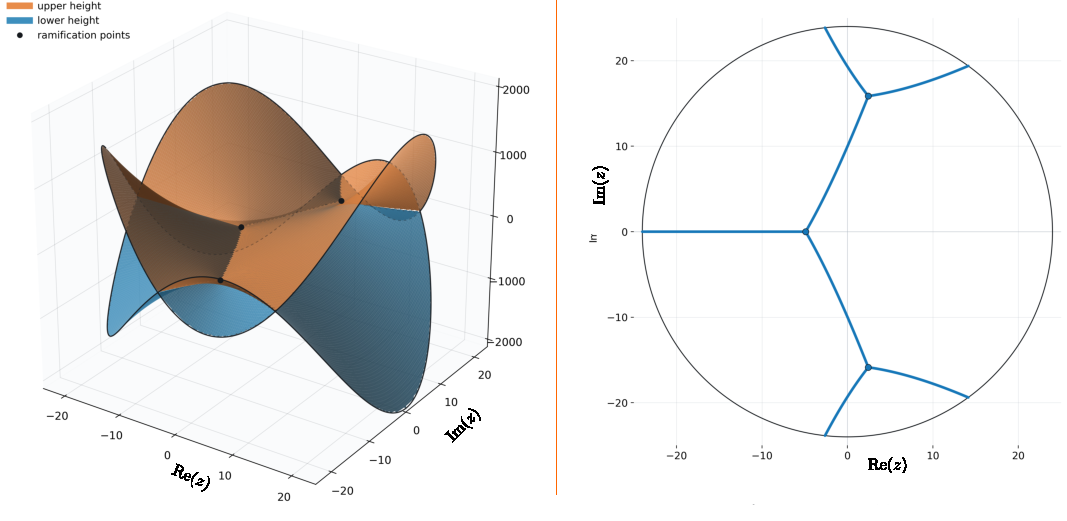
\includegraphics[width=\textwidth]{figures/Numerical_A2_Boutroux.pdf}
		\caption{(Left) The graph of the map $z\mapsto (z,\Re\left(\int w(z)dz\right))$, where $\tilde{f}(z,w(z))=0$ and $\tilde{f}(z,w)$ is the deformation of $w^2-z^3$ defined in \eqref{eq:Boutroux_A2_case}, as in \Cref{ex:special_fillings}.(2). (Right) The locus $\w\sse\R^2_{x_1,x_2}$ of points where $\Re\left(\int w(z)dz\right)$ assigns one value, instead of the generic two values that are assigned to the points $(x_1,x_2)$ on the complement of $\w$. Here we identify $\R^2\cong\C_z$ via $z=x_1+ix_2$.}
		\label{fig:Numerical_Trefoil_2weave}
	\end{figure}
\end{center}

\begin{remark}\label{rmk:Boutroux_via_period} As pointed out to me by Y.J.~Nho, for singularities of the form $z^2=w^{n+1}$, including \Cref{ex:special_fillings}.(2) above, one can argue the existence of a Morsification with purely imaginary $wdz$-periods by \cite[Theorem 1]{Varchenko1988}, though it does not provide explicit coefficients.\sbs
\end{remark}

\noindent As hopefully illustrated by \Cref{ex:special_fillings}, it is a rather subtle matter to use \Cref{lem:complex_curve_real_Lagrangian} to construct and easily manipulate embedded exact Lagrangian fillings coming from algebraic curves. From a geometric and topological viewpoint, there are two downsides:\\

\begin{enumerate}
    \item It can be challenging to geometrically visualize these surfaces in 4-dimensions.\\

    \item The rigidity of complex analysis and algebraic geometry makes it challenging to manipulate by hand these Lagrangian fillings. Specifically, in the spirit of geometric topology, with which contact and symplectic topology shares many features, it would be ideal to be able to construct and manipulate these Lagrangian fillings via local models and cut-and-paste arguments.\\
\end{enumerate}

\noindent We will now explain a solution to (1), which leads to considering the notion of a weave. Once weaves are defined, they immediately resolve (2) above. The idea to address (1) above is \Cref{rmk:Lagrangians_as_graphs} above. Namely, we insist on thinking of exact Lagrangians as graphs $\gr(df)\sse\R^4_{x_1,x_2,y_1,y_2}$, where $f:\R^2_{x_1,x_2}\lr\R$ is possibly multivalued. Such a primitive $f$ can be extracted from the exact Lagrangian itself by restricting $\la_\std$ (or a fixed ambient primitive) and integrating. In order to visualize exact Lagrangians, we plot the graph $\gr(f)\sse\R^3$, which is a singular surface in 3-dimensional space: this at least we can directly visualize with our eyes.

\begin{example}\label{ex:first_weave_plots} (1) Consider a smooth algebraic curve $\{(z,w)\in\C^2:P(z,w)=0\}\sse\C^2$. Then we can express $w=w(z)$ as a multivalued function of $z$ by requiring $P(z,w(z))=0$. Suppose the curve has purely imaginary $zdw$-periods. Then the associated exact Lagrangian surface in $(\D^4,\la_\std)$ can be understood as $\gr(df)$ where the multivalued function $f$ is
\begin{equation}\label{eq:graph_Re_integral}
f:\R^2_{x_1,x_2}\lr\R,\qquad f(x_1,x_2):=\Re\left(\int w(z)dz\right)
\end{equation}
where we write $z:=x_1+ix_2$ as above. Therefore, we can directly plot the graph of $z\mapsto (z,\Re(\int w(z)dz))$, which is a subset of $\R^3$.\footnote{Similarly, we could have instead expressed $z=z(w)$ as a multivalued function of $w$ by requiring $P(z(w),w)=0$ and plot the graph of $w\mapsto (w,\Re(\int z(w)dw))$.}\\

\noindent (2) Let us consider the $P(z,w):=\tilde{f}(z,w)$ as in \eqref{eq:Boutroux_A2_case} from \Cref{ex:special_fillings}.(2), which gives a Lagrangian filling of the Legendrian trefoil $\La_{\beta}$, with $\beta=\s_1^4$. In this case the graph of the multivalued function \eqref{eq:graph_Re_integral} is depicted in \Cref{fig:Numerical_Trefoil_2weave} (left). It can be described as follows:
\begin{enumerate}[label=$(\roman*)$]
    \item $f$ generically assigns 2 values per choice of $z=(x_1,x_2)\in\R^2$.\\
    \item There is a subset $\w\sse\R^2$ of points $(x_1,x_2)\in\R^2$ where $f$ assigns one value. This subset is depicted in \Cref{fig:Numerical_Trefoil_2weave} (right), as a subset of the $z$-plane, where $z=x_1+ix_2$.\\
    \item Within $\w$, there are 3 points where $\w$ is singular, each giving a trivalent vertex in $\w$. These are the three trivalent vertices depicted in \Cref{fig:Numerical_Trefoil_2weave} (right).
\end{enumerate}
\noindent The choice of notation $\w$ is no mistake. In summary, $\gr(f)\sse\R^3$ is a singular surface obtained by weaving two sheets in $\R^3$. The locus $\w$ records where these two sheets intersect. Generically they intersect at a codimension-one locus of immersed points, and within that locus there are three points with a more elaborate singularity. The name of this singularity is $D_4^-$, see \Cref{sssec:trivalent_model} below or \cite[Section 2.2.3]{CasalsWeng22}. The graphs for the variants \eqref{eq:Boutroux_A2_case_5symmetry} are obtained by rotating the plot by an angle of $2\pi/5$ in the base $z$-plane.\\

\begin{center}
	\begin{figure}[h!]
		\centering
		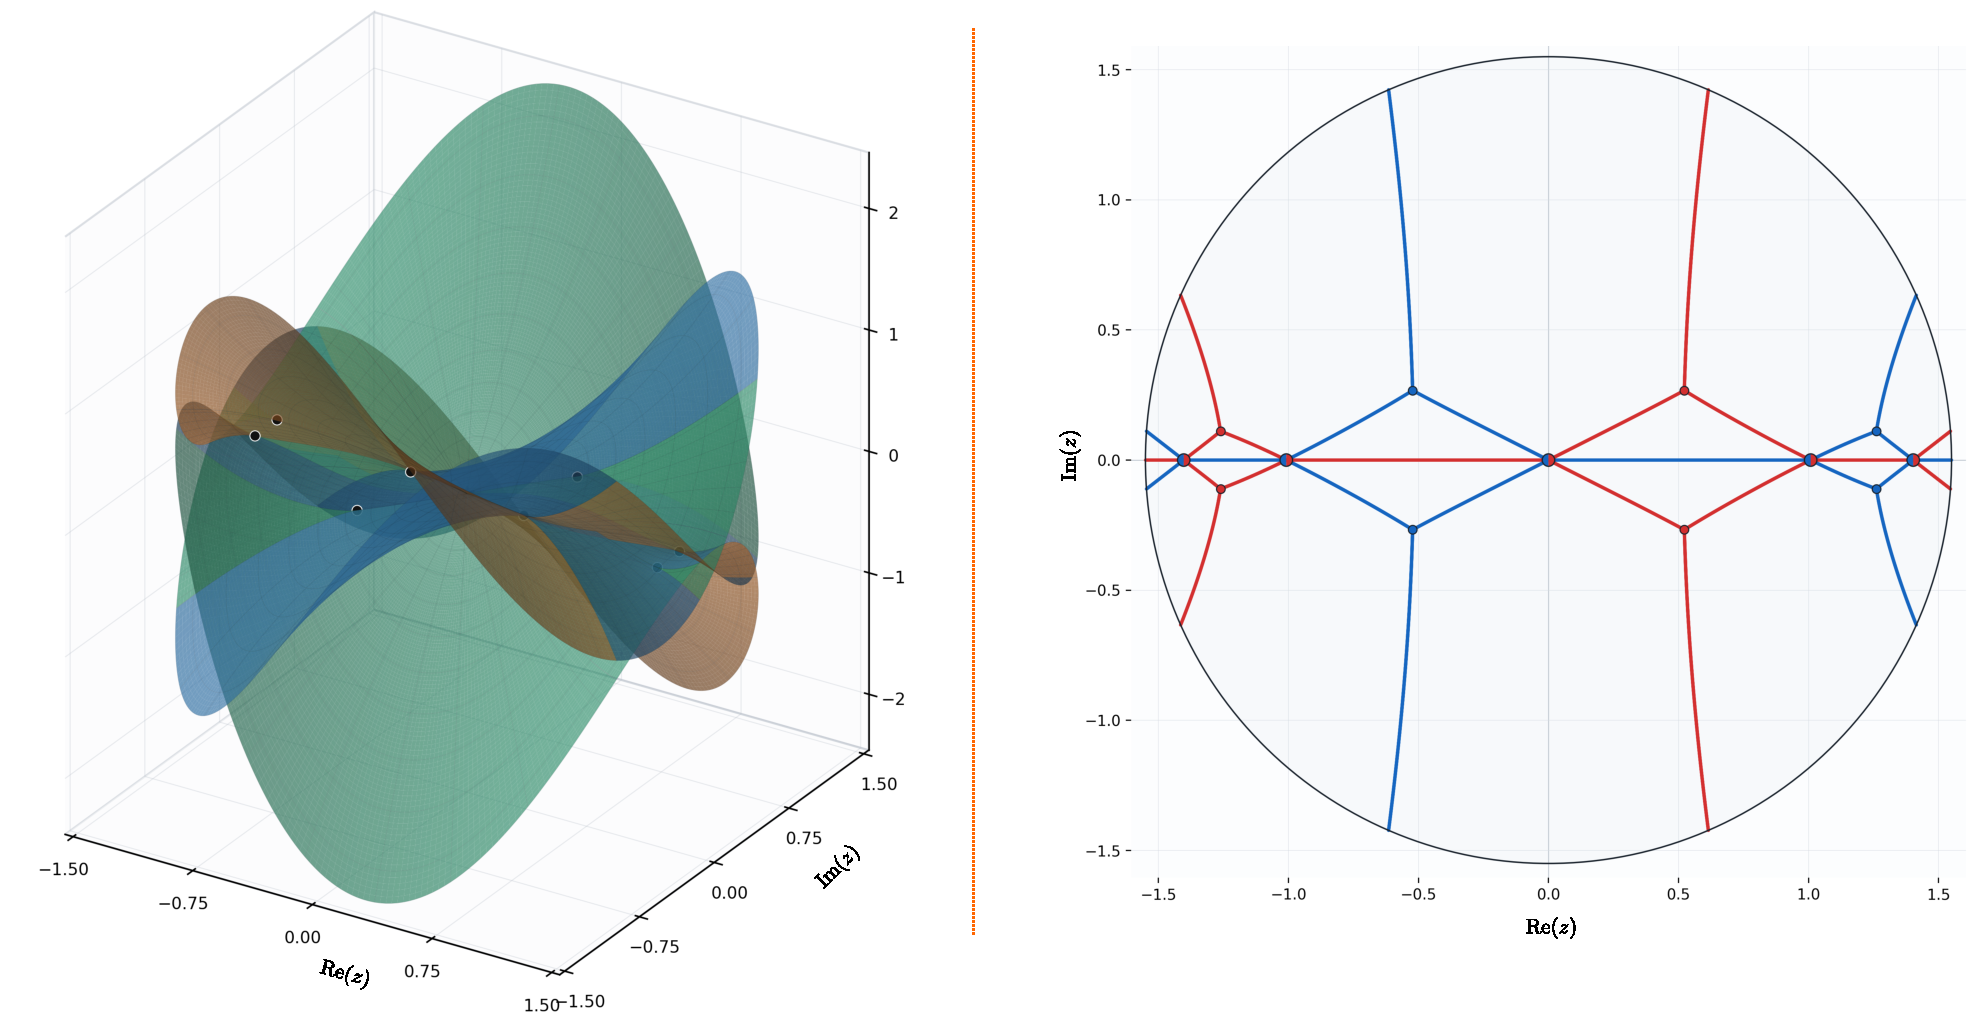
\includegraphics[width=\textwidth]{figures/Numerical_E6_Boutroux.pdf}
		\caption{(Left) The graph of the map $z\mapsto (z,\Re\left(\int w(z)dz\right))$, where $\tilde{f}(z,w(z))=0$ and the deformation $\tilde{f}(z,w)$ of $w^3-z^4$ is defined as in \eqref{eq:e6-fb}, cf.~\Cref{ex:special_fillings}.(3). (Right) The locus $\w\sse\R^2_{x_1,x_2}$ of points where $\Re\left(\int w(z)dz\right)$ assigns strictly fewer than 3 values. At the hexavalent vertices the function is univalued, at the rest of $\w$ it is bi-valued, and on the complement of $\w$ it is tri-valued. We have depicted the points in $\w$ where sheets one and two intersect in blue, while the points in $\w$ where sheets two and three intersect are drawn in red.}
		\label{fig:Numerical_34_3weave}
	\end{figure}
\end{center}

\noindent (3) Let us consider the $P(z,w):=\tilde{f}(z,w)$ as in \eqref{eq:e6-fb} from \Cref{ex:special_fillings}.(3), which gives a Lagrangian filling of the Legendrian $(3,4)$-torus knot $\La_{\beta}$, with $\beta=(\s_1\s_2)^5\s_1$. The graph of the corresponding multivalued function, as in \eqref{eq:graph_Re_integral}, is depicted in \Cref{fig:Numerical_34_3weave} (left). It is described as follows:
\begin{enumerate}[label=$(\roman*)$]
    \item $f$ generically assigns 3 values per choice of $z=(x_1,x_2)\in\R^2$.\\
    \item There is a subset $\w\sse\R^2$ of points $(x_1,x_2)\in\R^2$ where $f$ assigns one or two values (instead of three). This subset $\w$ is depicted in \Cref{fig:Numerical_34_3weave} (right) as a subset of the $(x_1,x_2)$-plane, equivalently the $z$-plane with $z=x_1+ix_2$.\\

    Above a point in $\R^2\setminus\w$, we order the sheets from top to bottom. At a smooth point of $\w$ two sheets intersect: either the bottom two sheets or the top two sheets. For clarity, we have drawn the points in $\w$ where the bottom two sheets intersect in blue, and the points in $\w$ where the top two sheets intersect in red.\\
    
    \item Within $\w$, there are 13 points where the locus $\w$ is singular. Of these points, 8 give trivalent vertices in $\w$, and 5 of them give hexavalent vertices in $\w$. These are illustrated in \Cref{fig:Numerical_34_3weave} (right) as well.\\
\end{enumerate}
\noindent In summary, $\gr(f)\sse\R^3$ is a singular surface obtained by weaving three sheets in $\R^3$. The locus $\w$ records where these three sheets intersect. As before, these sheets generically intersect at a codimension-one locus of immersed points, and within that locus there are points with two types of singularities. The first type is a $D_4^-$-singularity, as above, and gives the trivalent vertices of $\w$. In these $D_4^-$-singularities only two consecutive sheets interact, the third sheet is simply entirely above or below them. The second type is an $A_1^3$-singularity, where the three sheets together actually meet at a point: it is exactly the type of singularity formed by union of the coordinate planes in $\R^3$, see \Cref{sssec:hexavalent_local_model} below.\sbs
\end{example}

\noindent \Cref{ex:first_weave_plots} should give a strong indication of the geometric relation between weaves and Lagrangian fillings. Indeed, \Cref{fig:Numerical_Trefoil_2weave} (right) is an $\SL_2$ weave, which is actually a Demazure weave $\w:\beta\to\delta(\beta)$ for $\beta=\s_1^4$. \Cref{fig:Numerical_34_3weave} (right) depicts an $\SL_3$ weave, which can be turned into a Demazure weave $\w:\beta\to\delta(\beta)$ for $\beta=(\s_1\s_2)^5\s_1$. The next subsection will add the necessary definitions and details.\\

\begin{remark}
Informally said, \Cref{fig:Numerical_Trefoil_2weave} (right) and \Cref{fig:Numerical_34_3weave} (right) each record the graph on their left by looking at it straight from above and only drawing where the sheets intersect, using the color to indicate which pair of consecutive sheets is intersecting.\sbs
\end{remark}

For now, we note that one can obtain a positive braid word $\eta_\w$, up to cyclic reordering, by reading the edges of $\w$ that intersect a large enough circle in the $z$-plane and recording which sheets intersect. Specifically, if we number the sheets bottom to top in increasing order of height, the intersection of sheets $i$ and $i+1$ is labeled by $\s_i$. This produces a positive braid word $\eta_\w$, up to cyclic reordering. For instance, if we start at $(20,0)$ in \Cref{fig:Numerical_Trefoil_2weave} (right) and go around clockwise we obtain $\eta_\w=\s_1^5$. Note that this is exactly $\beta\delta(\beta)=\s_1^5$ for $\beta=\s_1^4$, as in \Cref{ex:special_fillings}.(2). Similarly, if we start at $(0,2)$ in \Cref{fig:Numerical_34_3weave} (right) and go around clockwise we obtain $\eta_\w=(\s_1\s_2)^7=\beta\delta(\beta)$ where $\beta=(\s_1\s_2)^5\s_1$, as in \Cref{ex:special_fillings}.(3). Note that the same procedure applied to a Demazure weave $\w:\beta\to\delta(\beta)$ indeed always gives $\eta_\w=\beta\delta(\beta)$.

\begin{remark}\label{rmk:topology_Lagrangian_filling}
The topology of these embedded exact Lagrangian fillings $L\sse(\D^4,\la_\std)$ that we are visualizing by plotting the graph of $\Re\left(\int w(z)dz\right)$ can be readily deduced as follows. The restriction to $L$ of the projection $\C^2_{z,w}\lr\C_z$ onto the $z$-plane is a simple branched cover, of order the number of sheets above a generic point of $z$. The trivalent vertices of $\w$ are precisely the branch points of such projection. By Riemann-Hurwitz, all that remains to determine the diffeomorphism type of $L$ is to compute the number of boundary components: this is given by the number of cycles in which the braid word $\eta_\w$ decomposes when projected to the permutation group. Note that this is independent of the cyclic representative. Thus one can readily obtain the genus and number of boundary components from the set $\w$ if we label its edges by which sheets are joined right above them.\sbs
\end{remark}

\begin{remark}\label{rmk:front_of_lift}
For experts, \Cref{fig:Numerical_Trefoil_2weave} (left) and \Cref{fig:Numerical_34_3weave} (left) are fronts for Legendrian lifts of the corresponding exact Lagrangian surfaces. A Legendrian front for a Legendrian surface generically has singularities in real codimension one, e.g.~edges of cusps, and swallowtail singularities. (Here $A_1^2$ is not technically counted as a singularity, as it is an immersed locus.) The conceptual reason none of these fronts coming from algebraic curves have these cusp edges or swallowtails is that they are the real part of the complex front for a complex Legendrian curve. Since the front singularities of a complex Legendrian curve must be in complex codimension one, they must be points. Therefore, their real parts will have fronts with singularities in real codimension two. By the classification of Legendrian front singularities for surfaces, cf.~\cite[Chapter 21]{ArnoldGuseinZadeVarchenko85_Vol1}, they must be $A_1^3$ and $D_4^-$ singularities.\sbs
\end{remark}